
Consider tilings $\{T\}$ of the tilted square $T_n = \{(x, y) : |x| + |y| \leq n + 1\}$ in $\R^2$ by horizontal and vertical dominos of length $2$ and width $1$. For each tiling the dominos must lie strictly within $T_n$. The tilings $T$ are called Aztec diamonds because the boundary of $T$ in $\{(x, y) : y > 0\}$, say, has the shape of a Mexican pyramid. It is a nontrivial theorem that for any $n$, the number of domino tilings of $T_n$ is $2^{n \choose 2}$ .
\begin{figure}[ht!]
	\centering
	\subfigure{
		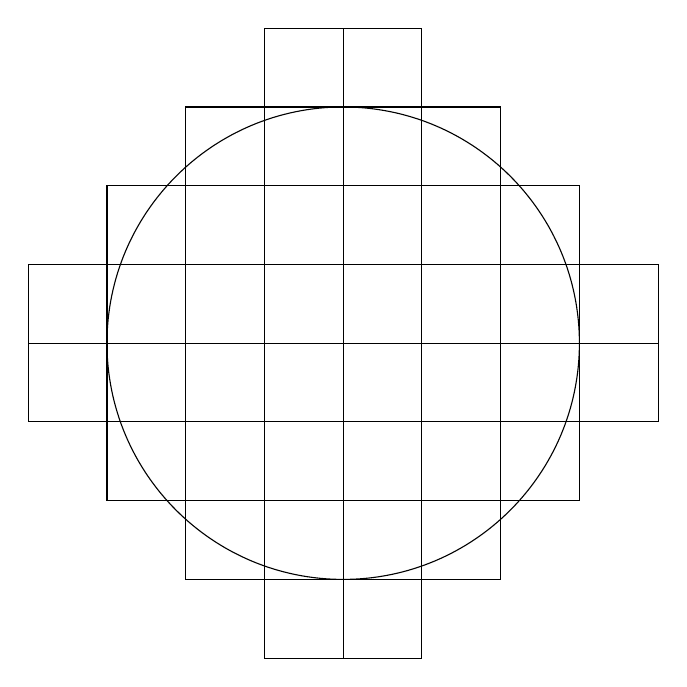
\begin{tikzpicture}[x=1cm]
			\foreach \y in {-5,...,5}{
				\foreach \x in {-5,...,5}{
					\pgfmathparse{abs(\y-0.5) + abs(\x-0.5)}
					\ifnum 5 > \pgfmathresult
					\draw (\x,\y) rectangle (\x,\y) rectangle (1+\x,1+\y);
					\fi
				}
			}
			\draw (1,1) circle (3);
		\end{tikzpicture}
	}
	\subfigure{
		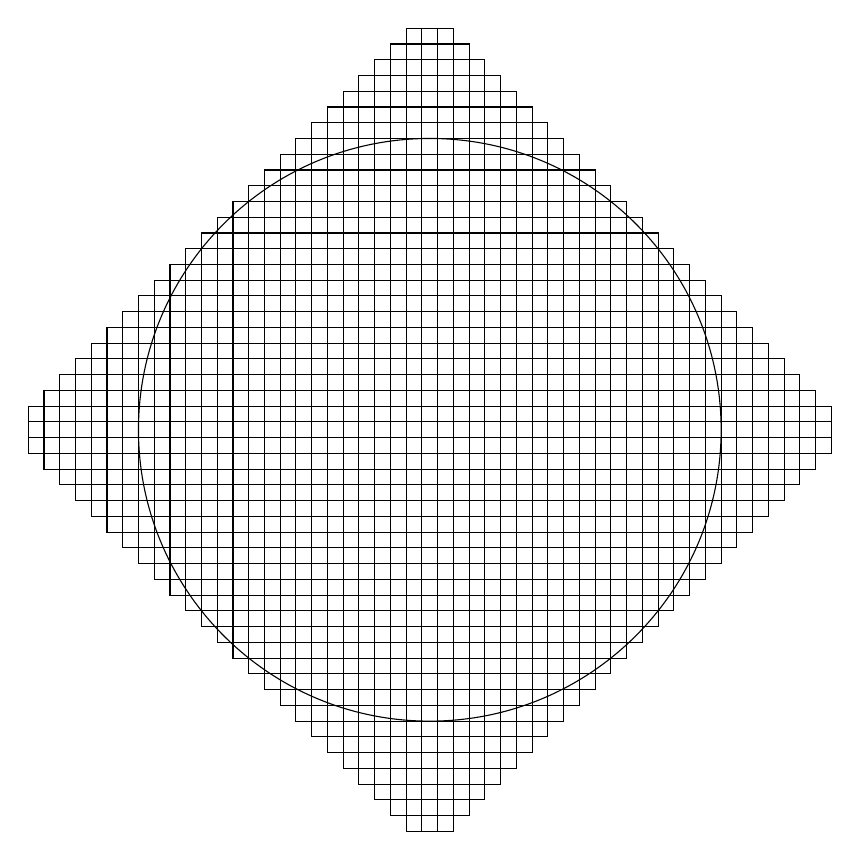
\begin{tikzpicture}[x=1cm]
			\foreach \y in {-25,...,25}{
				\foreach \x in {-25,...,25}{
					\pgfmathparse{abs(\y)-1 + abs(\x)-1}
					\ifnum 25 > \pgfmathresult
					\draw (\x /5, \y /5) rectangle ++(0.2,0.2);
					\fi
				}
			}
			\draw (0.1,0.1) circle (3.7);
		\end{tikzpicture}
	}
\end{figure}
Assume that all tilings are equally likely. The first thing one might notice when plotting tilings is that the most common tilings have a quirky behaviour: They freese the borders and stay random at a circle in the center.
\begin{figure}[h]
	\centering
	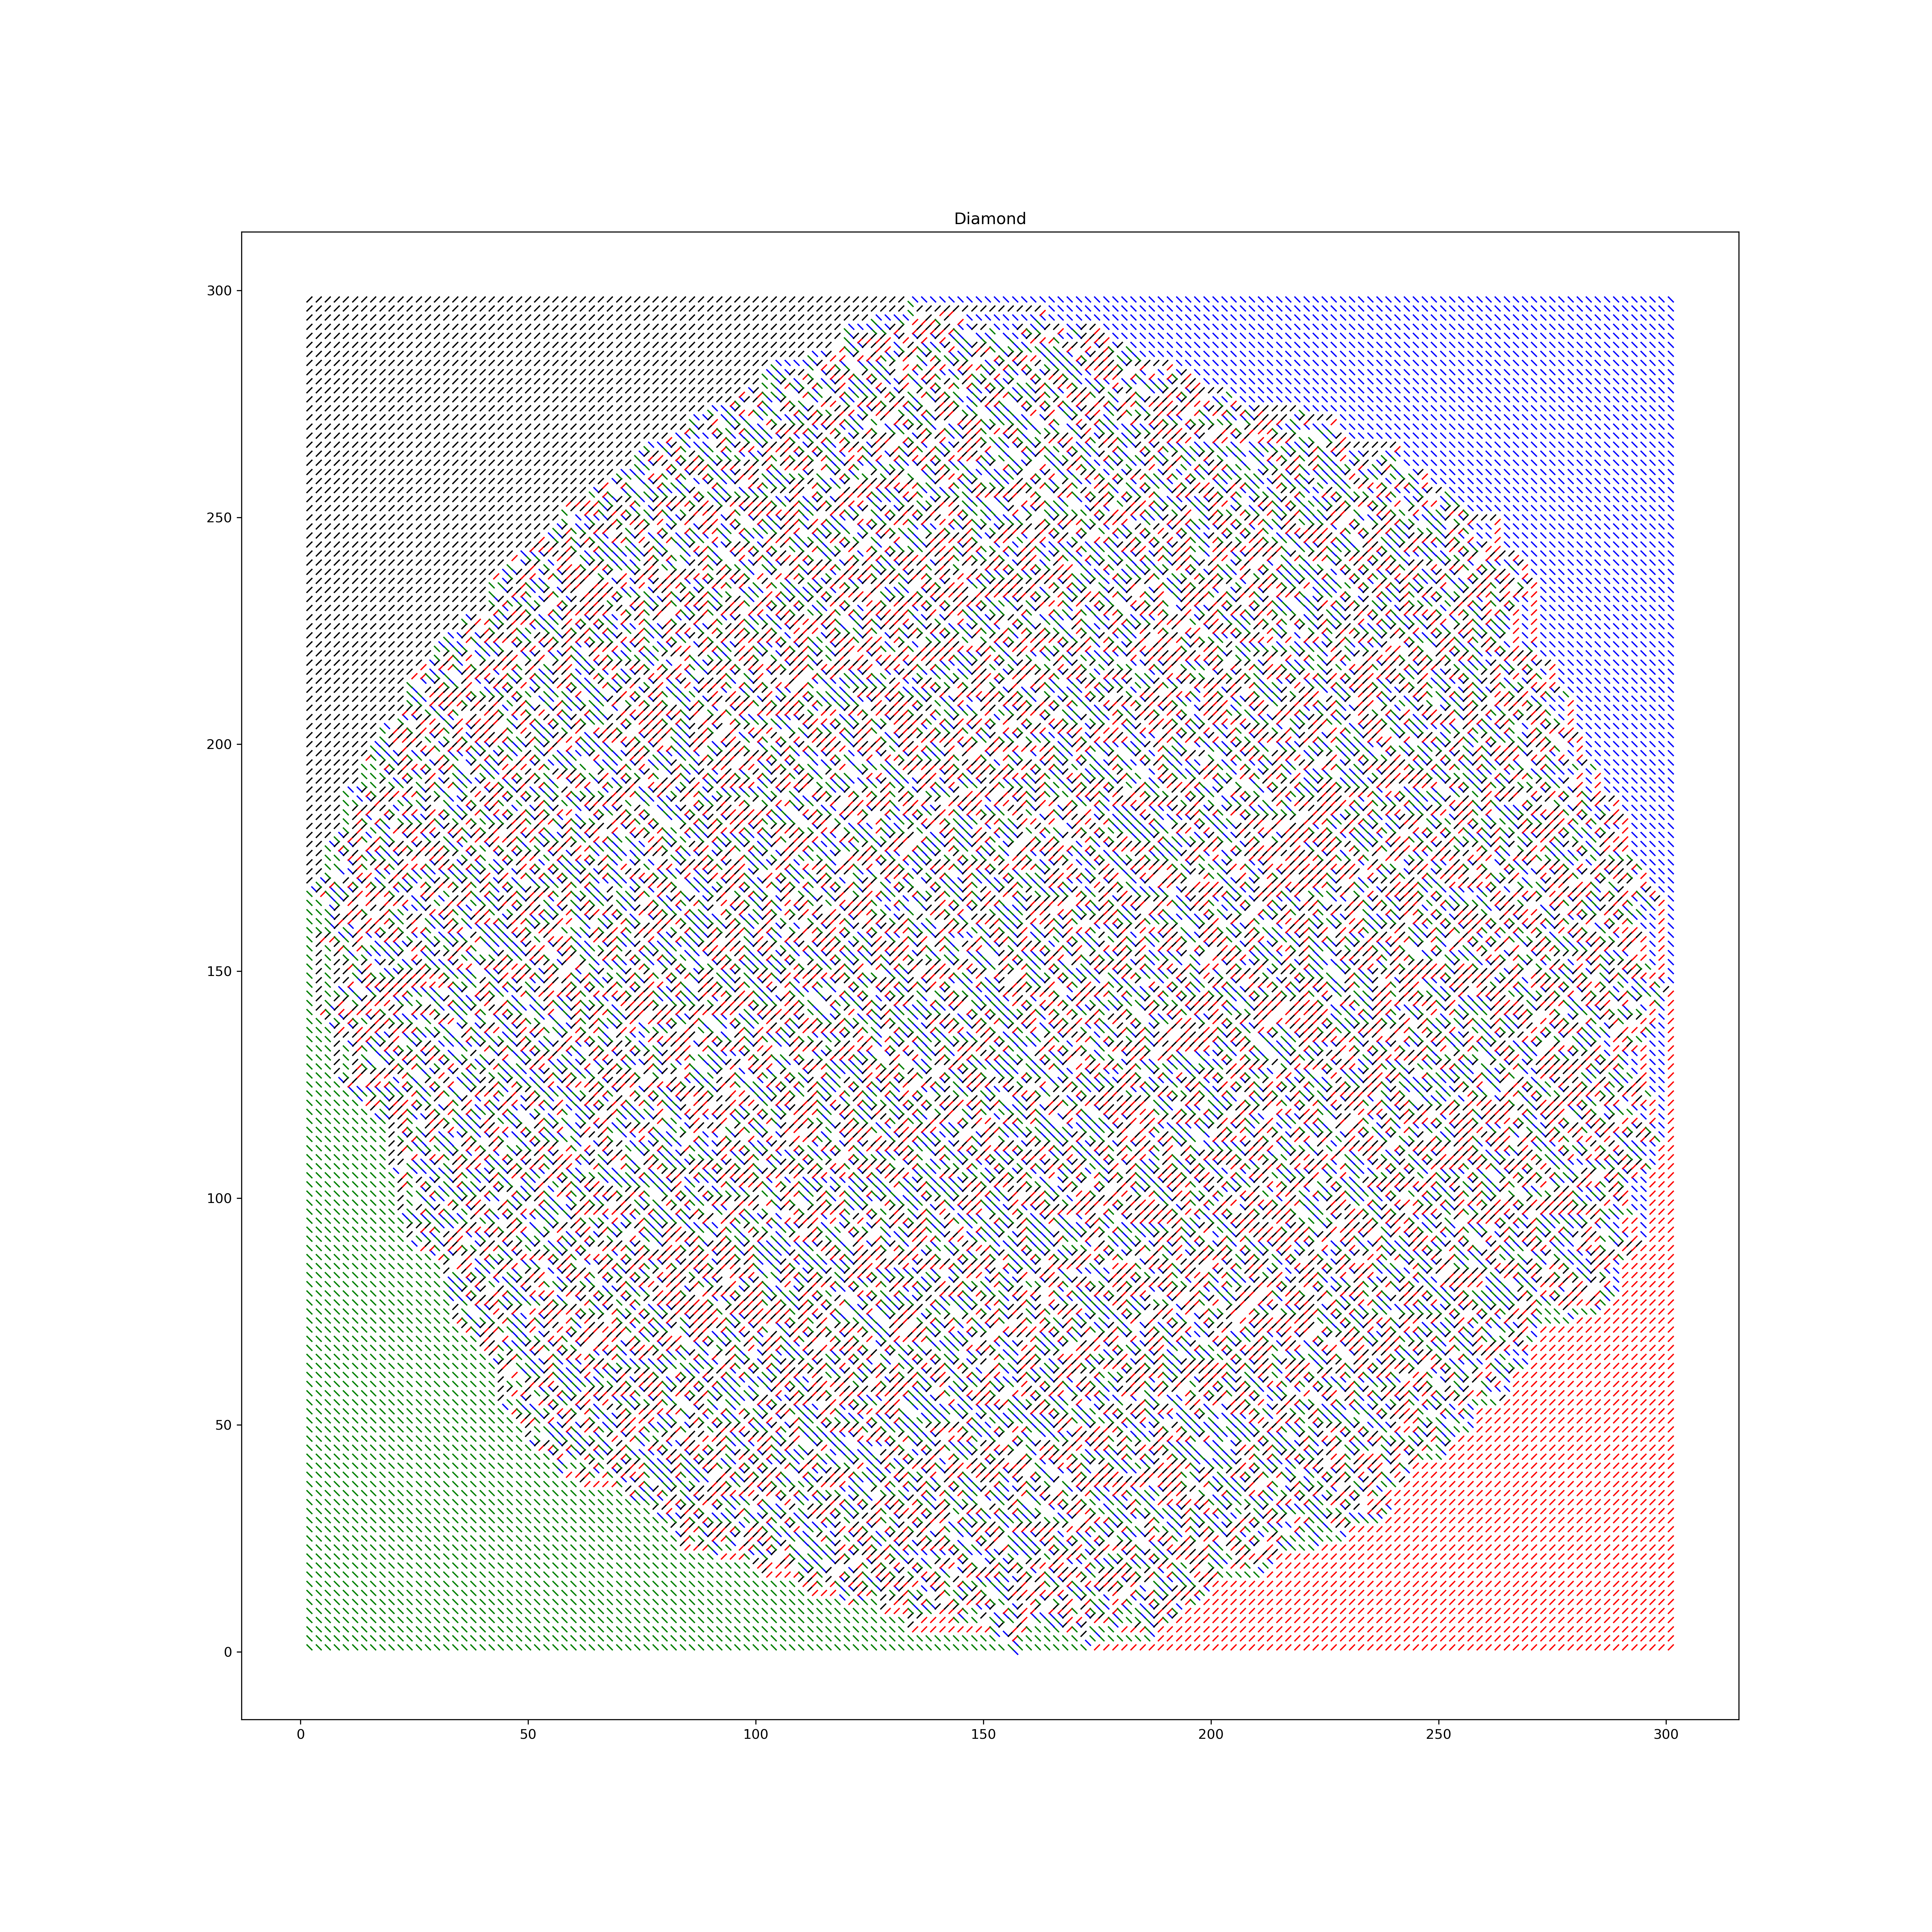
\includegraphics[width=0.7\linewidth]{./Assets/AstecDiamond.png}
\end{figure}
This is formally expressed in \cite{10.1214/10-AOP628}, 
\begin{thm}
	(The Article circle Theorem) FIz $\epsilon > 0$. FOr each $n$, consider a uniformly random domino tiling of the Astec Diamond of size $n$ scaçed by the factor $1/n$ in each axis to fit into the limiting diamond
	\begin{equation}
		AD_\infty \deff \{ |x| + |y| \leq 1\}
	\end{equation}
	and let $P_n^0 \subset n^{-1}AD_n$ be the image of the polar regions of the random tiling under this scaling transformation. Then as $n \rightarrow \infty$ the event that
	\begin{equation}
		\{(x, y) \in AD_\infty : x^2 + y^2 > \frac{1}{2} + \epsilon\} \bigcap (n^{-1} AD_n ) \subset P^0_n \subset \{(x, y) \in AD_\infty : x^2 + y^2 > \frac{1}{2} - \epsilon\}
	\end{equation}
	holds with probability that tends to $1$.
\end{thm}
The interesting result is in how much the border of the random region - or temperate, as some authors call it - deviates from the Artic Circle as $N$ grows large. For $-1 < \alpha < 1$ and $\alpha \neq 0$, let
\begin{equation}
	(x_\alpha^+, y_\alpha^+) = \left( 	\frac{\alpha + \sqrt{1-\alpha^2}}{2} , \frac{\alpha + \sqrt{1+\alpha^2}}{2}\right) \quad \text{and}, \quad (x_\alpha^-, y_\alpha^-) = \left( 	\frac{\alpha - \sqrt{1-\alpha^2}}{2} , \frac{\alpha + \sqrt{1+\alpha^2}}{2}\right) 
\end{equation}
denote the two points of intersection of the line $u + v = \alpha$ with $C_0 = \{u^2 + v^2 = \frac{1}{2}\}$. Then for fixed $\alpha$, Johansson showed that the fluctuations of the boundary of the temperate zone along the line $u + v = \alpha$ about the points $(x_\alpha^+ , y_\alpha^+ )$ and $(x_\alpha^- , y_\alpha^-)$ were described by the Tracy-Widom distribution $F_2$.